%% LyX 2.3.7 created this file.  For more info, see http://www.lyx.org/.
%% Do not edit unless you really know what you are doing.
\documentclass[english]{article}
\usepackage[T1]{fontenc}
\usepackage[latin9]{inputenc}
\usepackage[landscape]{geometry}
\geometry{verbose,tmargin=2cm,bmargin=2cm,lmargin=2cm,rmargin=2cm}
\usepackage{color}
\usepackage{array}
\usepackage{multirow}
\usepackage{footnote}
\usepackage{graphicx}

\makeatletter

%%%%%%%%%%%%%%%%%%%%%%%%%%%%%% LyX specific LaTeX commands.

\makesavenoteenv{tabular}

%% Special footnote code from the package 'stblftnt.sty'
%% Author: Robin Fairbairns -- Last revised Dec 13 1996
\let\SF@@footnote\footnote
\def\footnote{\ifx\protect\@typeset@protect
    \expandafter\SF@@footnote
  \else
    \expandafter\SF@gobble@opt
  \fi
}
\expandafter\def\csname SF@gobble@opt \endcsname{\@ifnextchar[%]
  \SF@gobble@twobracket
  \@gobble
}
\edef\SF@gobble@opt{\noexpand\protect
  \expandafter\noexpand\csname SF@gobble@opt \endcsname}
\def\SF@gobble@twobracket[#1]#2{}
%% Because html converters don't know tabularnewline
\providecommand{\tabularnewline}{\\}

\@ifundefined{showcaptionsetup}{}{%
 \PassOptionsToPackage{caption=false}{subfig}}
\usepackage{subfig}
\makeatother

\usepackage{babel}
\begin{document}

\section{Test matrices}

\begin{tabular}{|c|c|c|c|c|c|c|c|}
\hline 
Matrix & Patt. symm. & Num. symm. & Diag. dom. & Pos. def. & NNZ & $n$ & Condition\tabularnewline
\hline 
\hline 
\emph{add20} & 100\% & 52.7\% & No & No & 13,151 & 2,395 & 1.204710e+04\tabularnewline
\hline 
\emph{c-20} & 100\% & 100\% & No & No & 20,445 & 2,921 & 1.049837e+12\tabularnewline
\hline 
\emph{cryg2500} & 99.5\% & 0\% & No & No & 12,349 & 2,500 & 3.631392e+16\tabularnewline
\hline 
\emph{dw2048} & 98.5\% & 94.8\% & No & No & 10,114 & 2,048 & 2.093210e+03\tabularnewline
\hline 
\emph{orsreg\_1} & 100\% & 41.2\% & \textbf{Yes} & No & 14,133 & 2,204 & 6.745269e+03\tabularnewline
\hline 
\emph{pde2961} & 100\% & 50.1\% & No & No & 14,585 & 2,961 & 6.424933e+02\tabularnewline
\hline 
\emph{wang1} & 100\% & 80.8\% & No & No & 19,093 & 2,903 & 2.032301e+04\tabularnewline
\hline 
\textcolor{red}{ex28}\footnote{Preconditioners are singular, except for iLU(0).} & 100\% & 98.8\% & No & No & 77,031 & 2,603 & 1.983028e+05 \tabularnewline
\hline 
\textcolor{red}{gre512}\footnote{Preconditioners are singular, except for iLU(0).} & 0\% & 0\% & No & No & 1,976 & 512 & 1.58318e+02\tabularnewline
\hline 
\textcolor{red}{S40PI}\footnote{Preconditioners are singular.} & 100\% & 2.3\% & No & No & 5,341 & 2,182 & 3.851536e+18 \tabularnewline
\hline 
\end{tabular}

\section{$S$ coverage, degree\protect\footnote{$S$ degree := $\max_{i\in[n]}\left|\{j\mid A_{ij}\protect\neq0\}\right|-1$}}

\begin{minipage}[t]{0.5\columnwidth}%
\begin{tabular}{|c|c|c|c|c|c|}
\hline 
Matrix & jacobi & tridiag & maxLF & maxST & minST\tabularnewline
\hline 
\hline 
\emph{add20} & 0.5686 & 0.5698 & 0.9496 & 0.9997 & 0.6480\tabularnewline
\hline 
\emph{c-20} & 0.9994 & 0.9994 & 0.9996 & 0.9998 & 0.9996\tabularnewline
\hline 
\emph{cryg2500} & 0.5038 & 0.8796 & 0.9040 & 0.9064 & 0.5744\tabularnewline
\hline 
\emph{dw2048} & 0.5808 & 0.9140 & 0.9423 & 0.9437 & 0.6371\tabularnewline
\hline 
\emph{orsreg\_1} & 0.5001 & 0.5003 & 0.9949 & 0.9954 & 0.5017\tabularnewline
\hline 
\emph{pde2961} & 0.5027 & 0.6310 & 0.8730 & 0.8742 & 0.6370\tabularnewline
\hline 
\emph{wang1} & 0.5008 & 0.7422 & 0.8795 & 0.8905 & 0.5316\tabularnewline
\hline 
\textcolor{red}{ex28} & 0.3236 & 0.3311 & 0.6349 & 0.6588 & 0.3239\tabularnewline
\hline 
\textcolor{red}{gre512} & 0.1797 & 0.1816 & 0.4165 & 0.4292 & 0.4292\tabularnewline
\hline 
\textcolor{red}{S40PI} & 0.0486 & 0.9231 & 0.0703 & 0.0703 & 0.0703\tabularnewline
\hline 
\end{tabular}%
\end{minipage}\hfill{}%
\begin{minipage}[t]{0.5\columnwidth}%
\begin{tabular}{|c|c|c|c|c|c|c|}
\hline 
Matrix & orig & jacobi & tridiag & maxLF & maxST & minST\tabularnewline
\hline 
\hline 
\emph{add20} & 83 & \multirow{10}{*}{0} & \multirow{10}{*}{2} & \multirow{10}{*}{2} & 11 & 27\tabularnewline
\cline{1-2} \cline{2-2} \cline{6-7} \cline{7-7} 
\emph{c-20} & 157 &  &  &  & 148 & 40\tabularnewline
\cline{1-2} \cline{2-2} \cline{6-7} \cline{7-7} 
\emph{cryg2500} & 4 &  &  &  & 3 & 4\tabularnewline
\cline{1-2} \cline{2-2} \cline{6-7} \cline{7-7} 
\emph{dw2048} & 7 &  &  &  & 5 & 4\tabularnewline
\cline{1-2} \cline{2-2} \cline{6-7} \cline{7-7} 
\emph{orsreg\_1} & 6 &  &  &  & 3 & 4\tabularnewline
\cline{1-2} \cline{2-2} \cline{6-7} \cline{7-7} 
\emph{pde2961} & 4 &  &  &  & 3 & 3\tabularnewline
\cline{1-2} \cline{2-2} \cline{6-7} \cline{7-7} 
\emph{wang1} & 6 &  &  &  & 5 & 6\tabularnewline
\cline{1-2} \cline{2-2} \cline{6-7} \cline{7-7} 
\textcolor{red}{ex28} & 61 &  &  &  & 5 & 7\tabularnewline
\cline{1-2} \cline{2-2} \cline{6-7} \cline{7-7} 
\textcolor{red}{gre512} & 4 &  &  &  & 2 & 2\tabularnewline
\cline{1-2} \cline{2-2} \cline{6-7} \cline{7-7} 
\textcolor{red}{S40PI} & 6 &  &  &  & 2 & 2\tabularnewline
\hline 
\end{tabular}%
\end{minipage}

\section{Results}

\begin{figure}[h]
\begin{minipage}[t]{0.33\columnwidth}%
\subfloat[$x=1$]{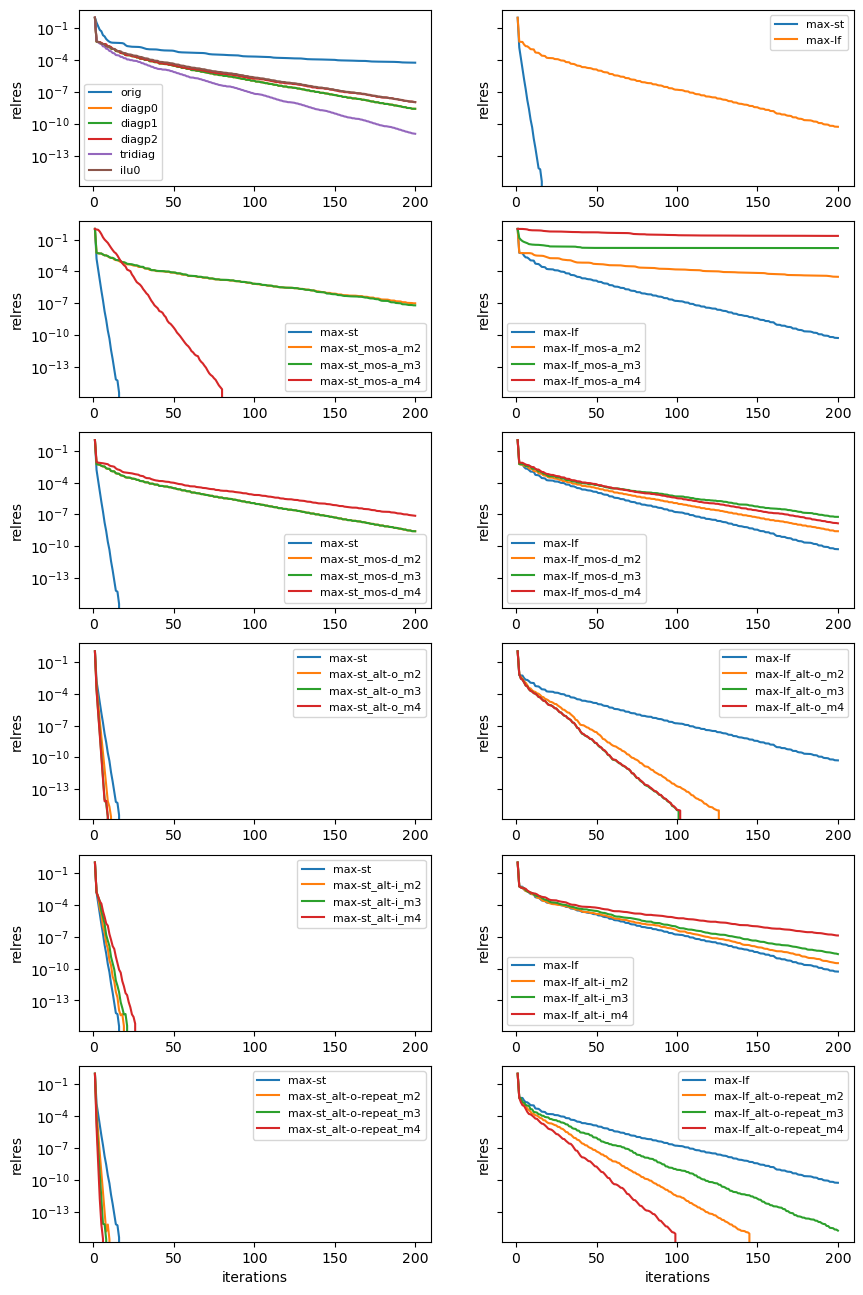
\includegraphics[width=1\textwidth]{png/add20_xones}

}%
\end{minipage}\hfill{}%
\begin{minipage}[t]{0.33\columnwidth}%
\subfloat[$x\sim\mathcal{N}(0,1)$]{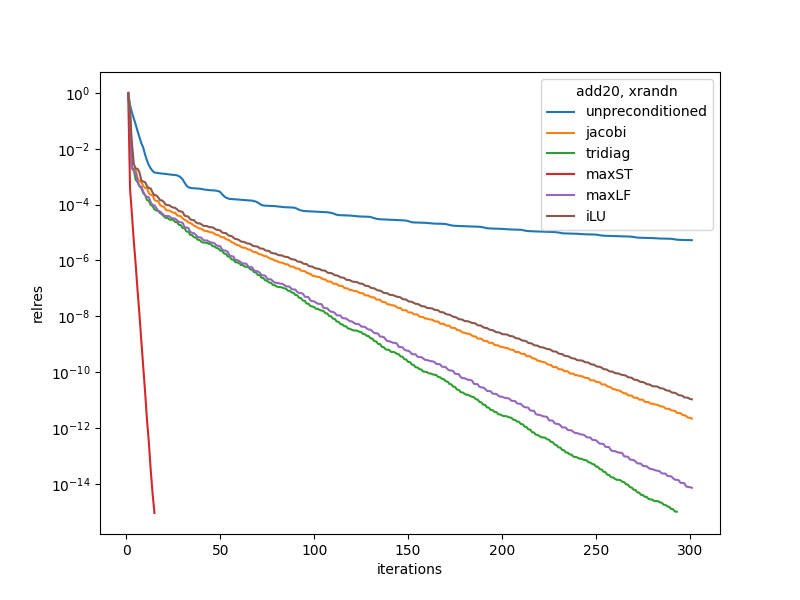
\includegraphics[width=1\textwidth]{png/add20_xrandn}

}%
\end{minipage}\hfill{}%
\begin{minipage}[t]{0.33\columnwidth}%
\subfloat[{$x=\sin([0,100\pi])$}]{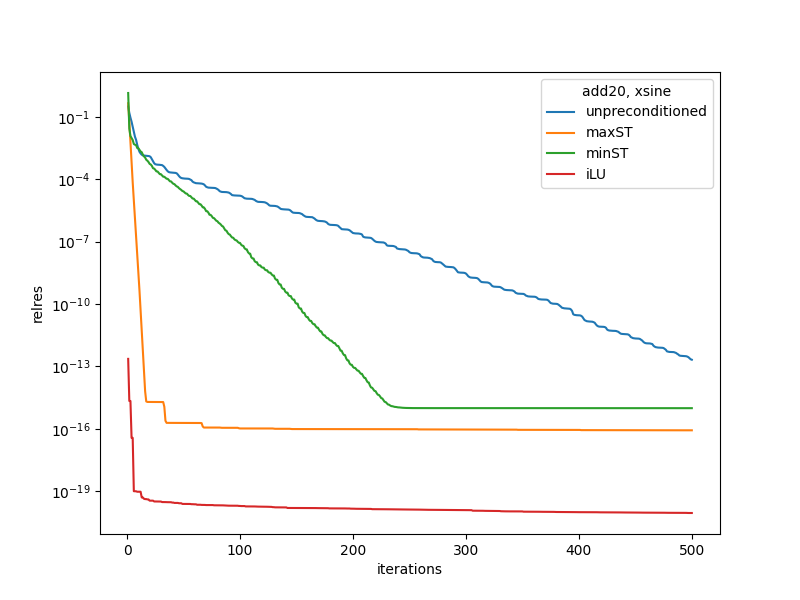
\includegraphics[width=1\textwidth]{png/add20_xsine}}%
\end{minipage}

\caption{add20}

\end{figure}

\begin{figure}[h]
\begin{minipage}[t]{0.33\columnwidth}%
\subfloat[$x=1$]{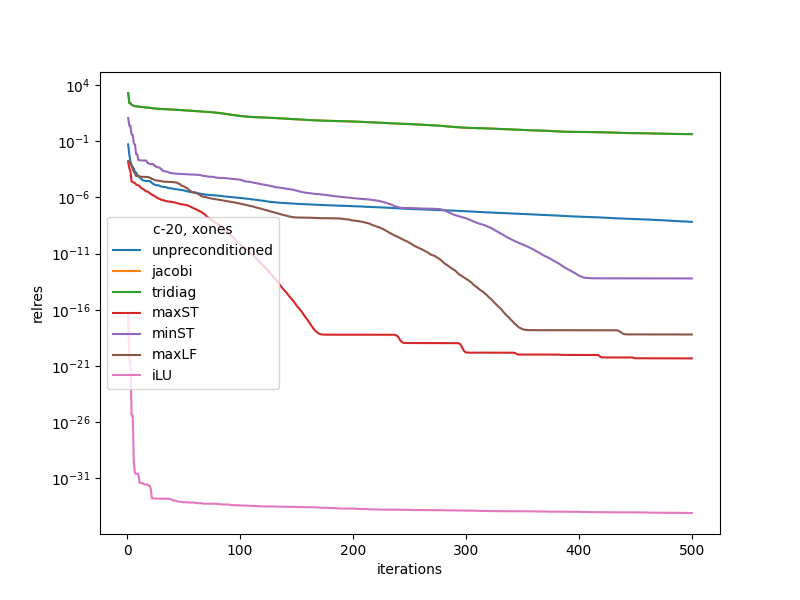
\includegraphics[width=1\textwidth]{png/c-20_xones}

}%
\end{minipage}\hfill{}%
\begin{minipage}[t]{0.33\columnwidth}%
\subfloat[$x\sim\mathcal{N}(0,1)$]{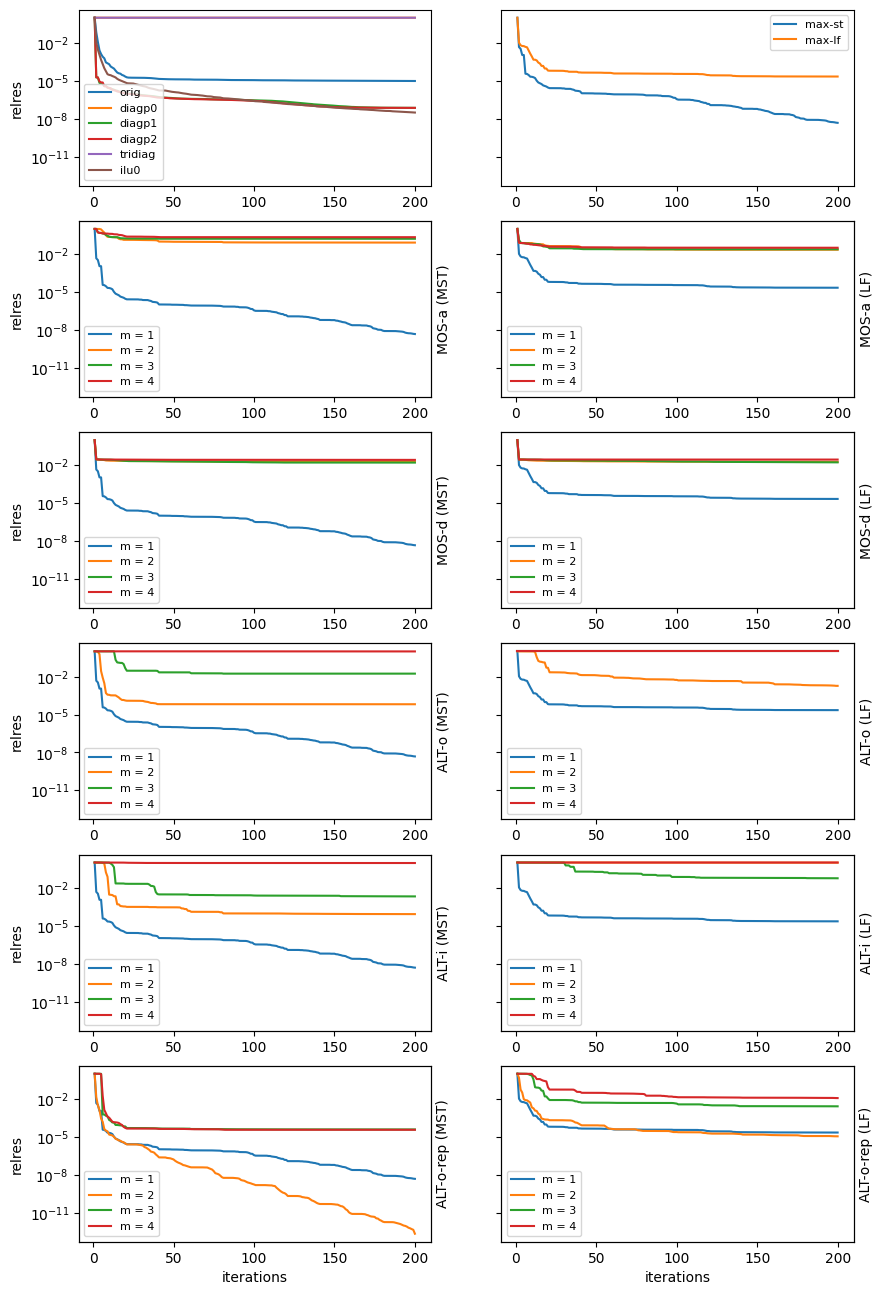
\includegraphics[width=1\textwidth]{png/c-20_xrandn}

}%
\end{minipage}\hfill{}%
\begin{minipage}[t]{0.33\columnwidth}%
\subfloat[{$x=\sin([0,100\pi])$}]{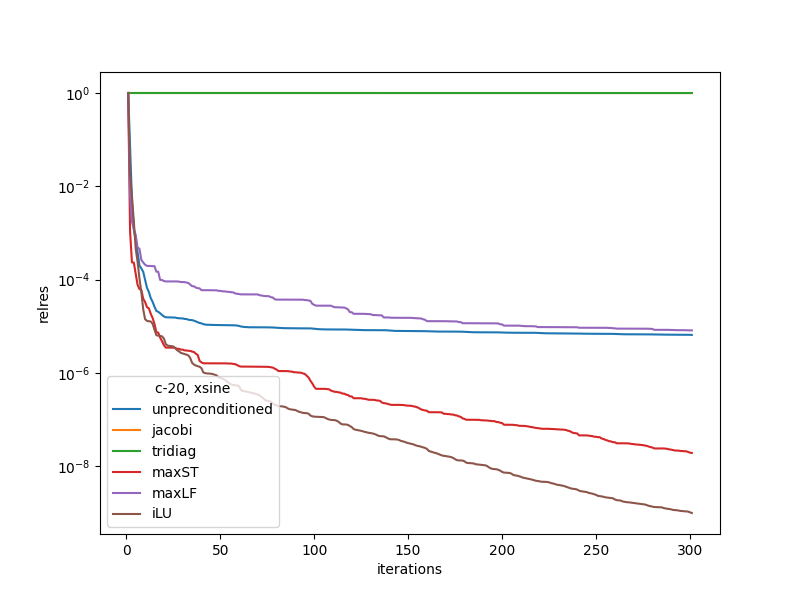
\includegraphics[width=1\textwidth]{png/c-20_xsine}}%
\end{minipage}

\caption{c-20}
\end{figure}

\begin{figure}[h]
\begin{minipage}[t]{0.33\columnwidth}%
\subfloat[$x=1$]{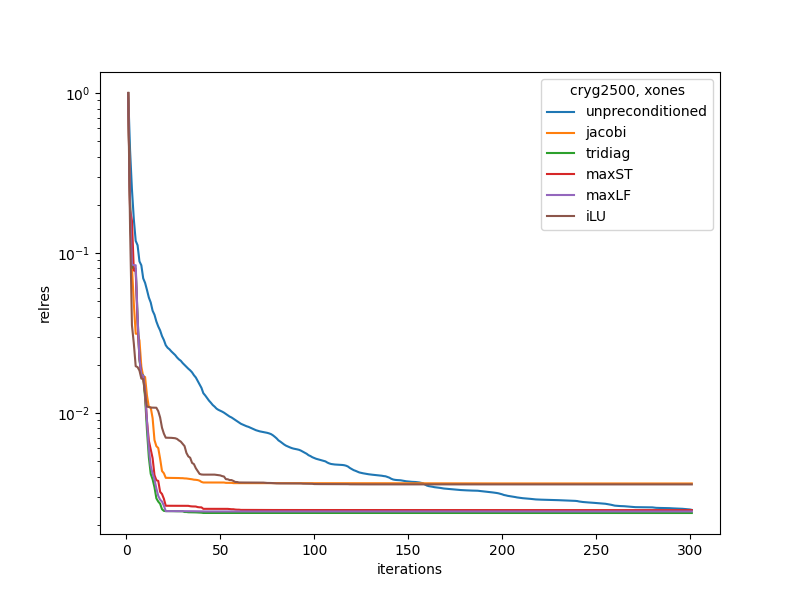
\includegraphics[width=1\textwidth]{png/cryg2500_xones}

}%
\end{minipage}\hfill{}%
\begin{minipage}[t]{0.33\columnwidth}%
\subfloat[$x\sim\mathcal{N}(0,1)$]{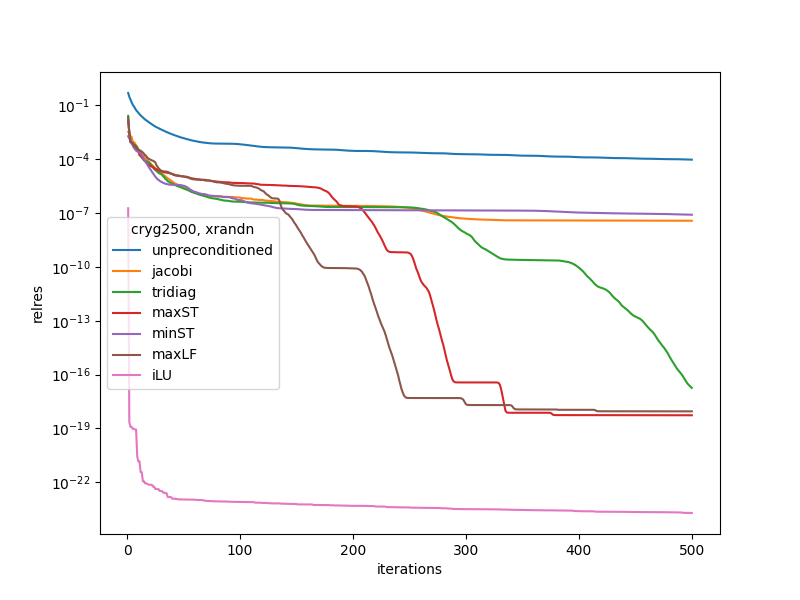
\includegraphics[width=1\textwidth]{png/cryg2500_xrandn}

}%
\end{minipage}\hfill{}%
\begin{minipage}[t]{0.33\columnwidth}%
\subfloat[{$x=\sin([0,100\pi])$}]{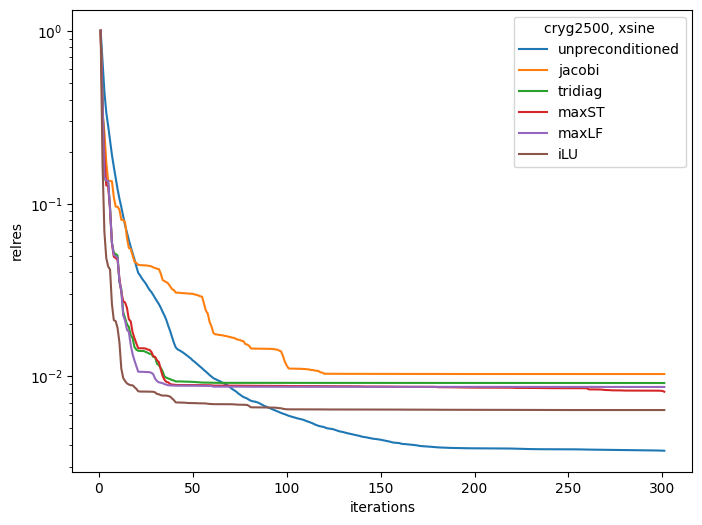
\includegraphics[width=1\textwidth]{png/cryg2500_xsine}}%
\end{minipage}

\caption{cryg2500}
\end{figure}

\begin{figure}[h]
\begin{minipage}[t]{0.33\columnwidth}%
\subfloat[$x=1$]{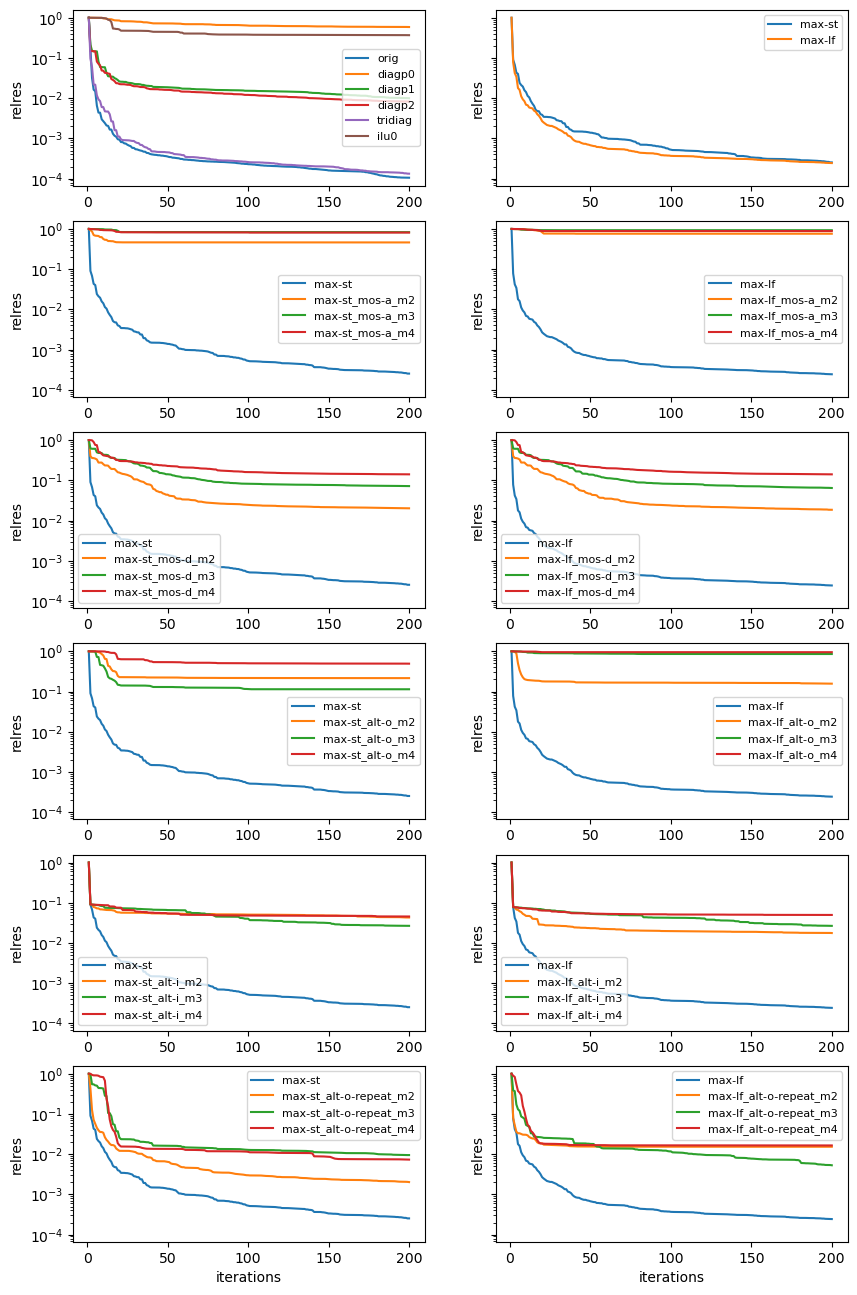
\includegraphics[width=1\textwidth]{png/dw2048_xones}

}%
\end{minipage}\hfill{}%
\begin{minipage}[t]{0.33\columnwidth}%
\subfloat[$x\sim\mathcal{N}(0,1)$]{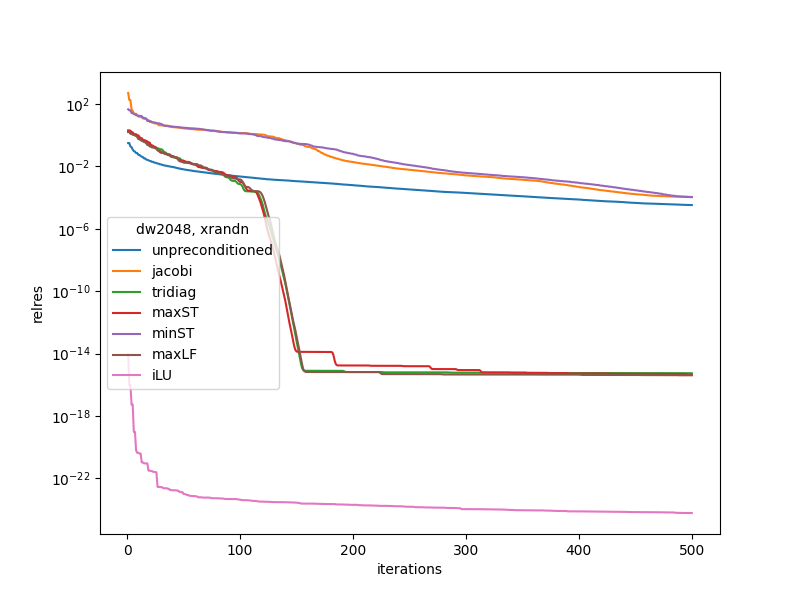
\includegraphics[width=1\textwidth]{png/dw2048_xrandn}

}%
\end{minipage}\hfill{}%
\begin{minipage}[t]{0.33\columnwidth}%
\subfloat[{$x=\sin([0,100\pi])$}]{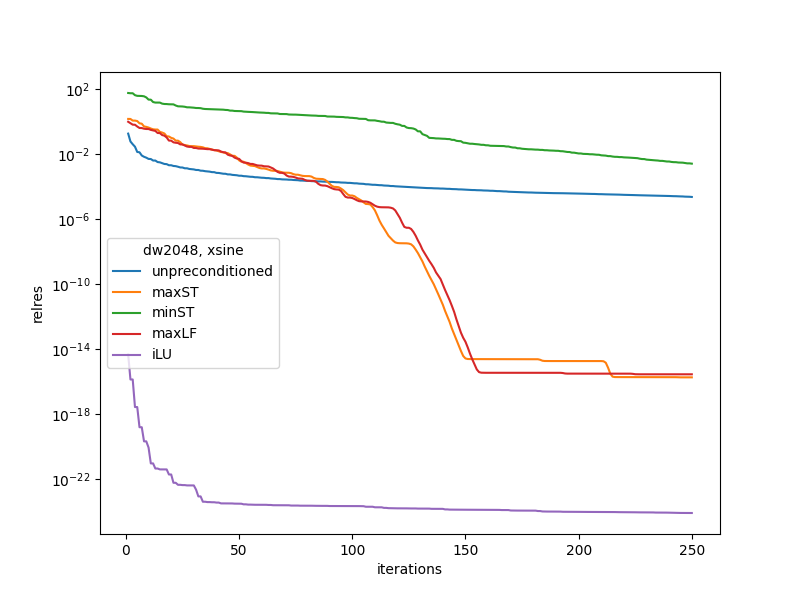
\includegraphics[width=1\textwidth]{png/dw2048_xsine}}%
\end{minipage}

\caption{dw2048}
\end{figure}

\begin{figure}[h]
\begin{minipage}[t]{0.33\columnwidth}%
\subfloat[$x=1$]{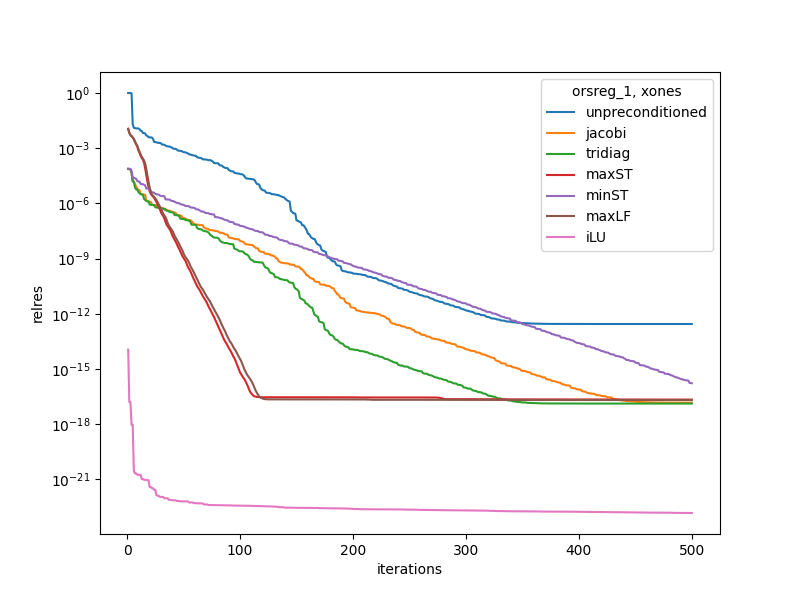
\includegraphics[width=1\textwidth]{png/orsreg_1_xones}

}%
\end{minipage}\hfill{}%
\begin{minipage}[t]{0.33\columnwidth}%
\subfloat[$x\sim\mathcal{N}(0,1)$]{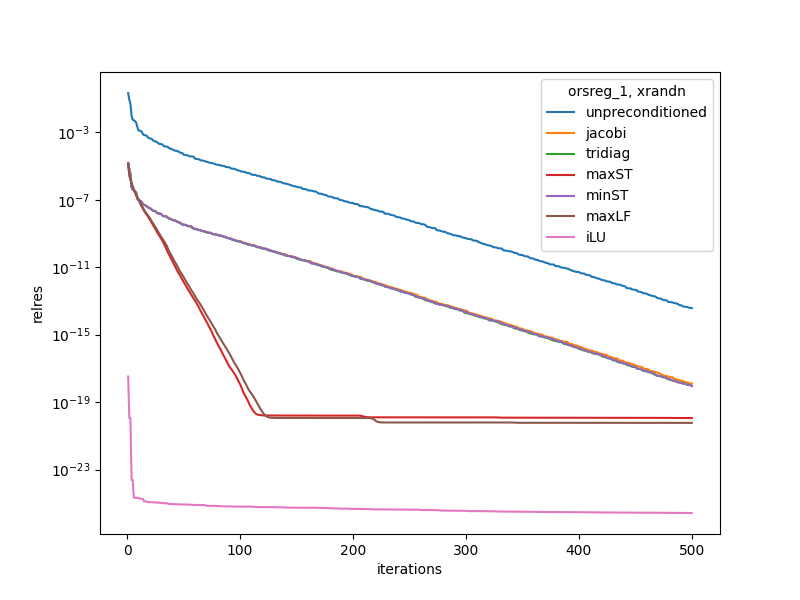
\includegraphics[width=1\textwidth]{png/orsreg_1_xrandn}

}%
\end{minipage}\hfill{}%
\begin{minipage}[t]{0.33\columnwidth}%
\subfloat[{$x=\sin([0,100\pi])$}]{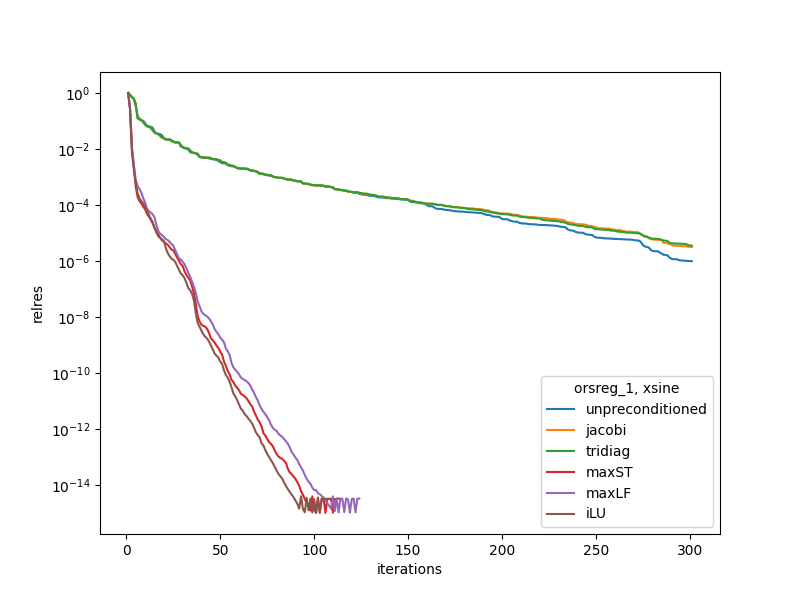
\includegraphics[width=1\textwidth]{png/orsreg_1_xsine}}%
\end{minipage}

\caption{orsreg\_1}
\end{figure}

\begin{figure}[h]
\begin{minipage}[t]{0.33\columnwidth}%
\subfloat[$x=1$]{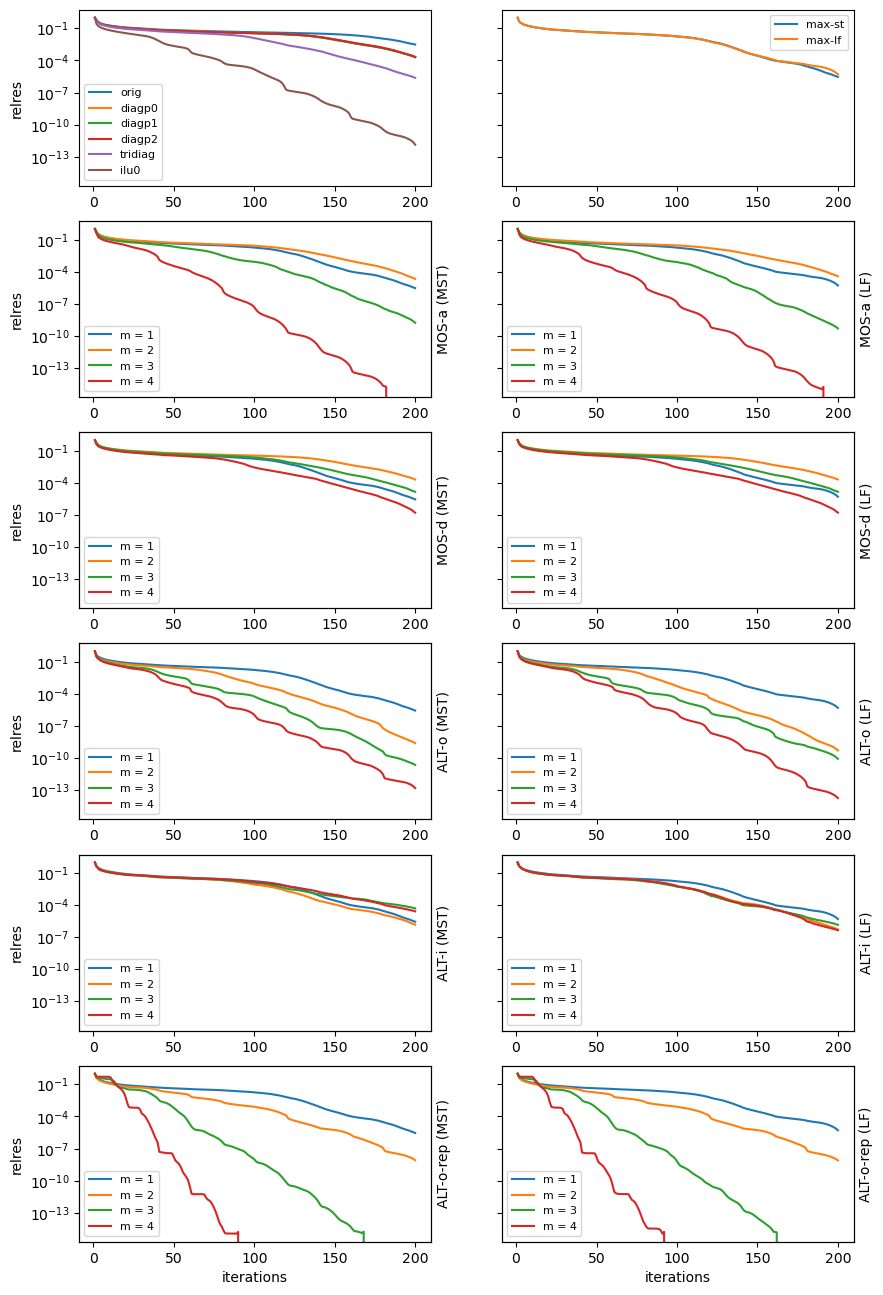
\includegraphics[width=1\textwidth]{png/pde2961_xones}

}%
\end{minipage}\hfill{}%
\begin{minipage}[t]{0.33\columnwidth}%
\subfloat[$x\sim\mathcal{N}(0,1)$]{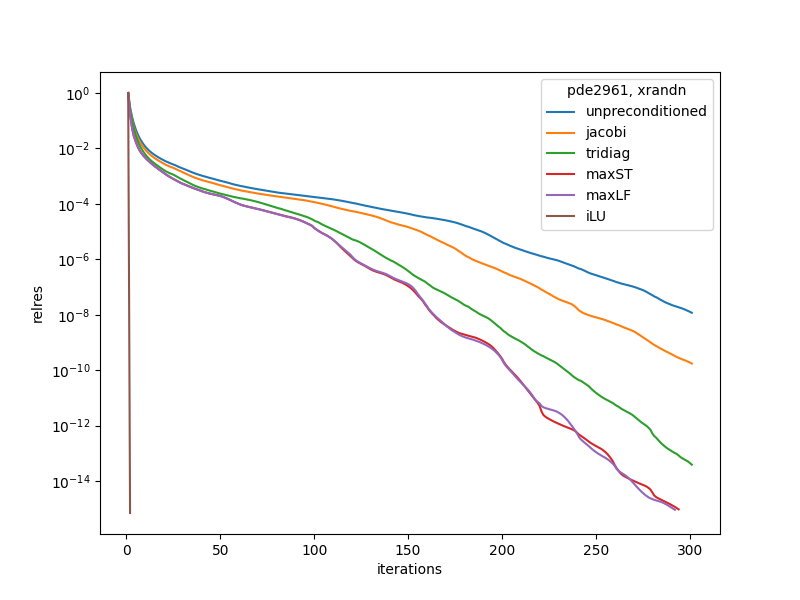
\includegraphics[width=1\textwidth]{png/pde2961_xrandn}

}%
\end{minipage}\hfill{}%
\begin{minipage}[t]{0.33\columnwidth}%
\subfloat[{$x=\sin([0,100\pi])$}]{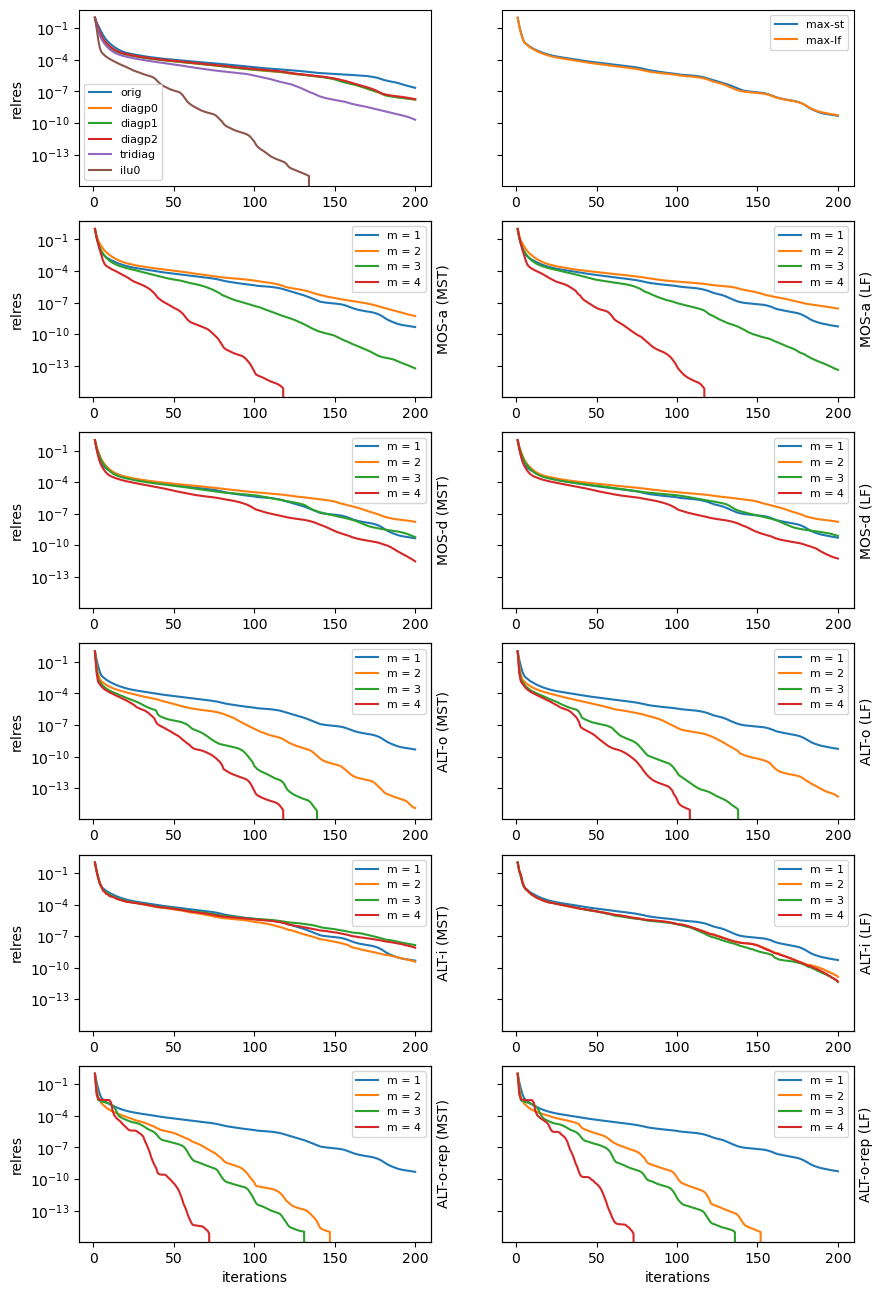
\includegraphics[width=1\textwidth]{png/pde2961_xsine}}%
\end{minipage}

\caption{pde2961}
\end{figure}

\begin{figure}[h]
\begin{minipage}[t]{0.33\columnwidth}%
\subfloat[$x=1$]{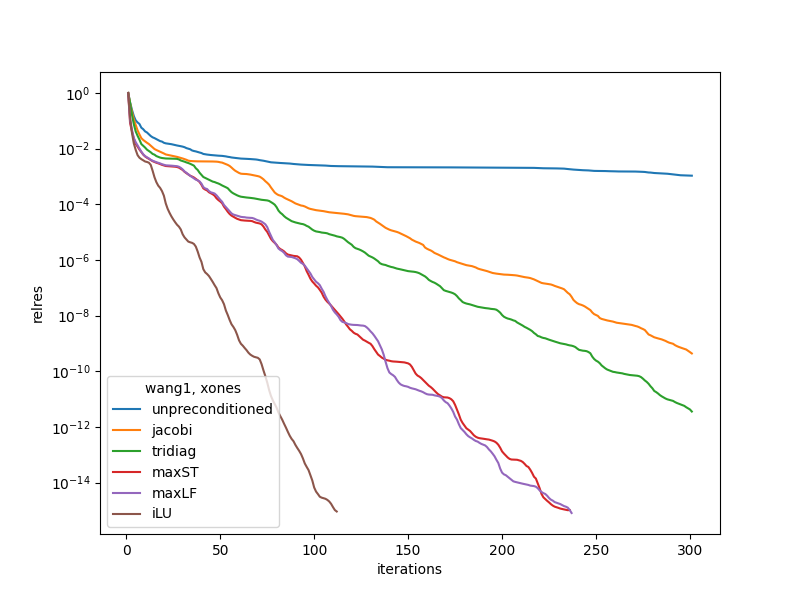
\includegraphics[width=1\textwidth]{png/wang1_xones}

}%
\end{minipage}\hfill{}%
\begin{minipage}[t]{0.33\columnwidth}%
\subfloat[$x\sim\mathcal{N}(0,1)$]{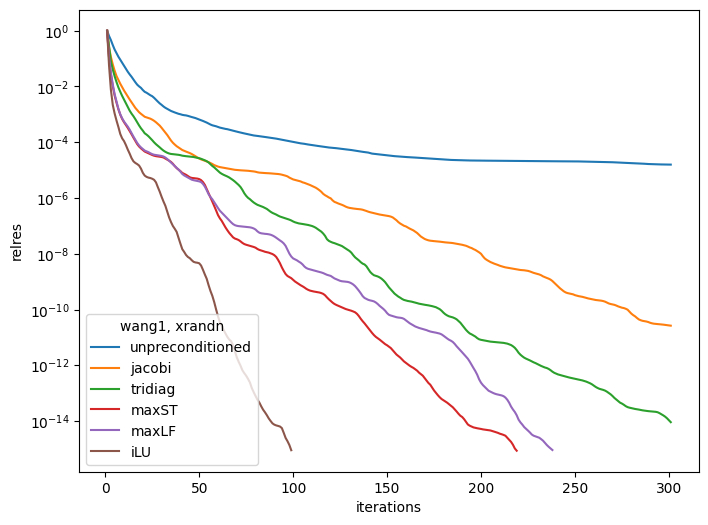
\includegraphics[width=1\textwidth]{png/wang1_xrandn}

}%
\end{minipage}\hfill{}%
\begin{minipage}[t]{0.33\columnwidth}%
\subfloat[{$x=\sin([0,100\pi])$}]{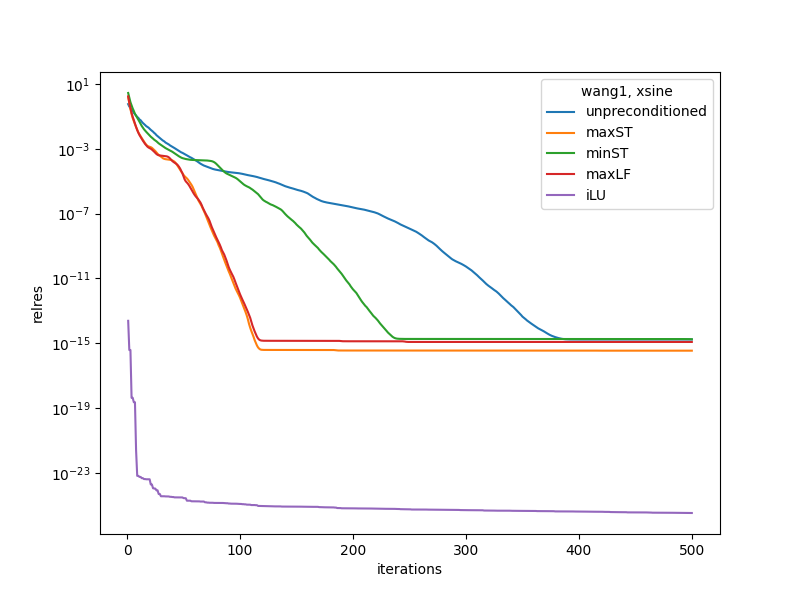
\includegraphics[width=1\textwidth]{png/wang1_xsine}}%
\end{minipage}

\caption{wang1}
\end{figure}

\end{document}
